\myframe{
  \ctr{Summary}
  \begin{itemize}
    \item Julia
    \item CUTEst
    \item Code fast and test
    \item Improve linear algebra
    \item Improve CUTEst calls
    \item Go down
  \end{itemize}
}

\myframe{
  \ctr{Julia}
  \begin{itemize}
    \item High level, High performance
    \item Great C/Fortran interface
    \item Easy syntax
  \end{itemize}
}

\begin{frame}[fragile]
  \ctr{Julia}
\begin{lstlisting}
$ julia
julia> A = rand(1000,1000);
julia> b = A*ones(1000);
julia> x = A\b;
julia> norm(A*x-b) + norm(x-ones(1000))
3.075209255065141e-11
\end{lstlisting}
\end{frame}

\begin{frame}[fragile]
  \ctr{Julia}
\begin{lstlisting}
julia> f(x) = x.^2
julia> t = rand(1000);
julia> y = [f(x) for x in t]
julia> z = zeros(t)
julia> for i = 1:length(t)
julia>     z[i] = f(t[i]);
julia> end
julia> w = f(t);
julia> norm(y-z)+norm(z-w)
0.0
\end{lstlisting}
\end{frame}

\myframe{
  \ctr{CUTEst}
  \begin{itemize}
    \item Repository of Nonlinear Optimization problems;
    \item Provides subroutines to obtain the problem informations;
    \item Decodes the problem, compiles your code with the problem's and run
      your main code;
    \item Widely used.
  \end{itemize}
}

\begin{frame}[fragile]
  \ctr{CUTEst}
\begin{lstlisting}
CALL cutest_cdimen(st, ifile, n, m)
if (m.GT.0) THEN
  STOP
ENDIF
CALL cutest_usetup(st, ifile, 7, 11, n, x, bl, bu)
CALL cutest_ufn(st, n, x, f)
\end{lstlisting}
\end{frame}

\begin{frame}[fragile]
  \ctr{CUTEst.jl}
  \begin{itemize}
    \item CUTEst interfaces in Julia
    \item Core interface
      \begin{lstlisting}
      CUTEst.ufn(st, n, x, f, libname)
      \end{lstlisting}
    \item Easy interface
      \begin{lstlisting}
      f = CUTEst.obj(nlp, x)
      \end{lstlisting}
  \end{itemize}
\end{frame}

\newcommand{\testerrorfix}[2]{
  \node[draw,rectangle,right of={#1},node distance=12em] (test) {Test};
  \draw[->] (#1) to[out=0,in=180] (test);
  \draw[->,dashed] (test) to[out=200,in=-4] (#1);
  \draw[->] (test) to[out=200,in=4] (#2);
}
\begin{frame}
  \ctr{Workflow}
  \begin{center}
  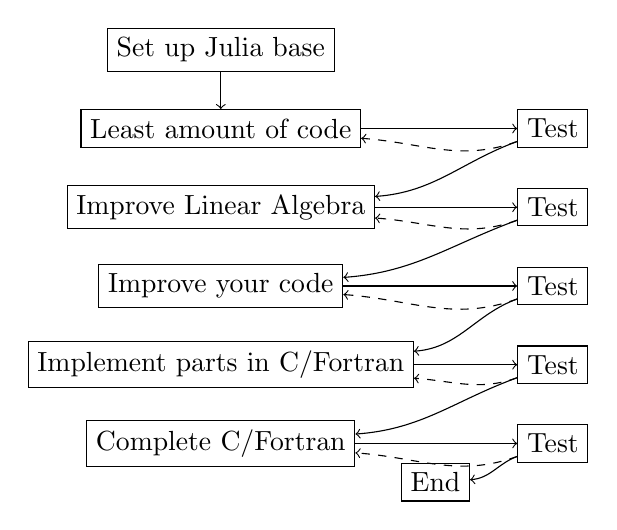
\begin{tikzpicture}
    \node[draw,rectangle] (start) {Least amount of code};
    \node[draw,rectangle,above of=start] (base) {Set up Julia base};
    \onslide<2->{
      \node[draw,rectangle,below of=start] (impLA) {Improve Linear Algebra};
      \testerrorfix{start}{impLA}
    }
    \onslide<3->{
      \node[draw,rectangle,below of=impLA] (impcode) {Improve your code};
      \testerrorfix{impLA}{impcode}
    }
    \onslide<4->{
      \node[draw,rectangle,below of=impcode] (lowlevel) {Implement parts in
        C/Fortran};
      \testerrorfix{impcode}{lowlevel}
    }
    \onslide<5->{
      \node[draw,rectangle,below of=lowlevel] (lowlevel2) {Complete C/Fortran};
      \testerrorfix{lowlevel}{lowlevel2}
    }
    \draw[->] (base) -- (start);

    \onslide<6->{ \node[draw,rectangle,below left of=test,node distance=6em]
        (end) {End};
      \testerrorfix{lowlevel2}{end};
    }
  \end{tikzpicture}
  \end{center}
\end{frame}
